\begin{pastexam}[label={px:ust-110-ee-ds-08}]{臺聯大電機類 110 學年度 第 8 題}
（問答）

(5\%) (a) Propose two graph storage structures for the graph in Figure 1 and explain the pros and cons
for those two structures.

(5\%) (b) Develop a minimal spanning tree of the graph.

\begin{center}
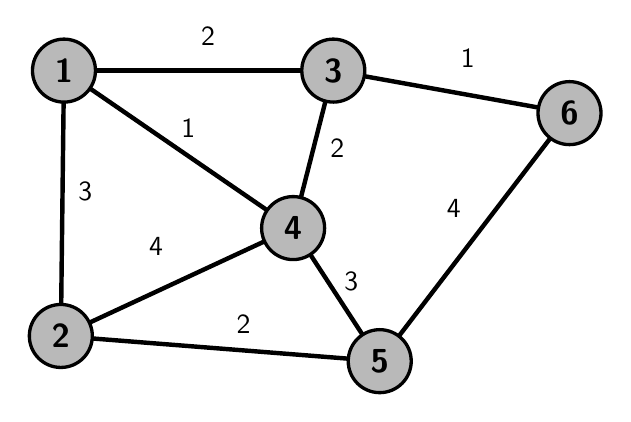
\begin{tikzpicture}[n/.style={circle,draw,line width=1.2pt,fill=gray!55,inner sep=0pt,minimum size=8mm,font=\large\bfseries\sffamily},w/.style={font=\sffamily,inner sep=0pt}]
\draw[line width=1.6pt] (1.32,-1.01)--(4.74,-1.01);
\node[w] at (3.15,-0.58) {2};
\draw[line width=1.6pt] (4.74,-1.01)--(7.74,-1.55);
\node[w] at (6.45,-0.85) {1};
\draw[line width=1.6pt] (1.32,-1.01)--(4.23,-3.01);
\node[w] at (2.90,-1.75) {1};
\draw[line width=1.6pt] (4.74,-1.01)--(4.23,-3.01);
\node[w] at (4.79,-2.00) {2};
\draw[line width=1.6pt] (1.32,-1.01)--(1.28,-4.38);
\node[w] at (1.59,-2.54) {3};
\draw[line width=1.6pt] (1.28,-4.38)--(4.23,-3.01);
\node[w] at (2.49,-3.24) {4};
\draw[line width=1.6pt] (4.23,-3.01)--(5.33,-4.70);
\node[w] at (4.97,-3.69) {3};
\draw[line width=1.6pt] (1.28,-4.38)--(5.33,-4.70);
\node[w] at (3.60,-4.23) {2};
\draw[line width=1.6pt] (7.74,-1.55)--(5.33,-4.70);
\node[w] at (6.27,-2.76) {4};
\node[n] at (1.32,-1.01) {1};
\node[n] at (4.74,-1.01) {3};
\node[n] at (7.74,-1.55) {6};
\node[n] at (4.23,-3.01) {4};
\node[n] at (1.28,-4.38) {2};
\node[n] at (5.33,-4.70) {5};
\end{tikzpicture}\\[2pt] Figure 1. Graph with weights.\end{center}
\end{pastexam}

\begin{pastsoln}
(a) 屬於資結書第~21~章（圖的表示法），(b) 屬於第~24~章（最小生成樹），本題放在第~24~章。

答案：(a) 相鄰矩陣和相鄰串列，見下；(b) 最小生成樹的總權重是 $9$，例如
$\{(1,4), (3,6), (1,3), (2,5), (1,2)\}$。 最小生成樹不唯一，共有 $4$ 棵，權重都是 $9$。

圖有 $n = 6$ 個頂點、$m = 9$ 條邊：$(1,2)\,3$、$(1,3)\,2$、$(1,4)\,1$、$(2,4)\,4$、$(2,5)\,2$、
$(3,4)\,2$、$(3,6)\,1$、$(4,5)\,3$、$(5,6)\,4$。

\textbf{(a) 相鄰矩陣。} $6 \times 6$ 的陣列，$M[u][v]$ 存邊 $(u, v)$ 的權重，沒有邊記 $\infty$，對角線
記 $0$。 無向圖所以對稱。
\[
M = \begin{array}{c|cccccc}
 & 1 & 2 & 3 & 4 & 5 & 6 \\ \hline
1 & 0 & 3 & 2 & 1 & \infty & \infty \\
2 & 3 & 0 & \infty & 4 & 2 & \infty \\
3 & 2 & \infty & 0 & 2 & \infty & 1 \\
4 & 1 & 4 & 2 & 0 & 3 & \infty \\
5 & \infty & 2 & \infty & 3 & 0 & 4 \\
6 & \infty & \infty & 1 & \infty & 4 & 0
\end{array}
\]

\textbf{相鄰串列。} 每個頂點一條串列，節點存（鄰居，權重）：
\begin{center}
\begin{tabular}{ll}
1: & $(2,3) \to (3,2) \to (4,1)$ \\
2: & $(1,3) \to (4,4) \to (5,2)$ \\
3: & $(1,2) \to (4,2) \to (6,1)$ \\
4: & $(1,1) \to (2,4) \to (3,2) \to (5,3)$ \\
5: & $(2,2) \to (4,3) \to (6,4)$ \\
6: & $(3,1) \to (5,4)$
\end{tabular}
\end{center}
每條邊在兩端各出現一次，共 $2m = 18$ 個節點。

\textbf{優缺點。}
\begin{itemize}
\item 相鄰矩陣：空間 $\Theta(n^2)$，這裡 $36$ 格，其中 $18$ 格有邊。 優點是查「$u$、$v$ 之間有沒有邊、權重
多少」$\Theta(1)$，寫法簡單。 缺點是空間和邊數無關，稀疏圖很浪費；列出一個頂點的鄰居要掃整列 $\Theta(n)$，
所以 BFS、DFS、Prim（陣列版）都是 $\Theta(n^2)$。
\item 相鄰串列：空間 $\Theta(n + m)$，稀疏圖省很多。 列出 $u$ 的鄰居是 $\Theta(\deg u)$，走訪整張圖
$\Theta(n + m)$。 缺點是查某一條邊要掃串列 $\Theta(\deg u)$；每個節點多一個指標，邊很多（稠密圖）時反而
比矩陣大。
\end{itemize}
這張圖 $n = 6$、$m = 9$，兩種都可以；一般原則是稠密圖用矩陣、稀疏圖用串列（資結書第~21.2~節）。

\textbf{(b)} 用 Kruskal 演算法（資結書第~24.2~節）：邊照權重由小到大排，權重相同時照端點編號，依序看，
不會形成環就加入。
\begin{center}
\begin{tabular}{clll}
\toprule
步 & 邊（權重） & 動作 & 加入後的連通塊 \\
\midrule
1 & $(1,4)$ 1 & 加入 & $\{1,4\}$ $\{2\}$ $\{3\}$ $\{5\}$ $\{6\}$ \\
2 & $(3,6)$ 1 & 加入 & $\{1,4\}$ $\{3,6\}$ $\{2\}$ $\{5\}$ \\
3 & $(1,3)$ 2 & 加入 & $\{1,3,4,6\}$ $\{2\}$ $\{5\}$ \\
4 & $(2,5)$ 2 & 加入 & $\{1,3,4,6\}$ $\{2,5\}$ \\
5 & $(3,4)$ 2 & 捨去（$3$、$4$ 已連通，會成環） & 不變 \\
6 & $(1,2)$ 3 & 加入 & $\{1,2,3,4,5,6\}$ \\
\bottomrule
\end{tabular}
\end{center}
已經有 $n - 1 = 5$ 條邊，停止。 總權重 $1 + 1 + 2 + 2 + 3 = 9$。

\begin{center}
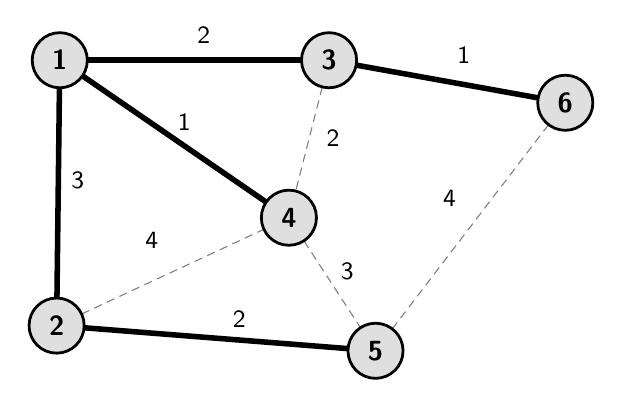
\begin{tikzpicture}[n/.style={circle,draw,line width=1pt,fill=gray!25,inner sep=0pt,minimum size=7mm,font=\bfseries\sffamily},w/.style={font=\sffamily\small,inner sep=0pt},t/.style={line width=2pt},o/.style={densely dashed,gray}]
\draw[t] (1.32,-1.01)--(4.74,-1.01);
\node[w] at (3.15,-0.70) {2};
\draw[t] (4.74,-1.01)--(7.74,-1.55);
\node[w] at (6.45,-0.95) {1};
\draw[t] (1.32,-1.01)--(4.23,-3.01);
\node[w] at (2.90,-1.80) {1};
\draw[o] (4.74,-1.01)--(4.23,-3.01);
\node[w] at (4.79,-2.00) {2};
\draw[t] (1.32,-1.01)--(1.28,-4.38);
\node[w] at (1.55,-2.54) {3};
\draw[o] (1.28,-4.38)--(4.23,-3.01);
\node[w] at (2.49,-3.30) {4};
\draw[o] (4.23,-3.01)--(5.33,-4.70);
\node[w] at (4.97,-3.69) {3};
\draw[t] (1.28,-4.38)--(5.33,-4.70);
\node[w] at (3.60,-4.30) {2};
\draw[o] (7.74,-1.55)--(5.33,-4.70);
\node[w] at (6.27,-2.76) {4};
\node[n] at (1.32,-1.01) {1};
\node[n] at (4.74,-1.01) {3};
\node[n] at (7.74,-1.55) {6};
\node[n] at (4.23,-3.01) {4};
\node[n] at (1.28,-4.38) {2};
\node[n] at (5.33,-4.70) {5};
\end{tikzpicture}

粗線是最小生成樹的邊，虛線是沒用到的邊。
\end{center}

\textbf{不唯一。} 第 3 步和第 5 步的 $(1,3)$、$(3,4)$ 權重都是 $2$，選誰都一樣，只要兩條不同時選（同時選
會和 $(1,4)$ 成環）；第 6 步的 $(1,2)$ 和還沒看到的 $(4,5)$ 權重都是 $3$，都能把 $\{2,5\}$ 接上。 所以共
$2 \times 2 = 4$ 棵最小生成樹，權重都是 $9$。 用 Prim 演算法從頂點 $1$ 出發也會得到權重 $9$ 的樹：依序加入
$(1,4)\,1$、$(1,3)\,2$（或 $(4,3)\,2$）、$(3,6)\,1$、$(1,2)\,3$（或 $(4,5)\,3$）、$(2,5)\,2$（或 $(5,2)\,2$）。
\end{pastsoln}
